\section{Results}

We conduct \gid{TODO \#EXP} experiments to investigate the performance of the 
proposed SOM algorithm. The first experiment tests the ability of a
two-dimensional map to learn representations of one-dimensional data.
Then we put the model on test on higher-dimensional data, and finally we
study the ability of the proposed algorithm to coping with degenerative
cases where either neurons are removed from the map or new units are added 
to the map. In these cases, the map has to undergo a reorganization to 
update the representations of the input space. \gid{TODO We could make a connection
to neuroscience here}. 
For every experiment we measure \gid{TODO ADD HERE THE ASSESSMENT MEASURES}. 

\subsection{One-dimensional data}

In the first experiment we use $50000$ samples drawn from a uniform distribution
($\mathcal{U}(0, 1)$) to train a two-dimensional map consists of $1024$ units
(neurons) for $25000$ epochs (all the parameters can be found in
Table~\ref{table:parameters}). Figure~\ref{fig:one-dim}{\bfseries \sffamily A}
shows the neural space topology of the two-dimensional map after sampling a 
blue noise distribution and placing the neurons on the corresponding nodes.
Figure~\ref{fig:one-dim}{\bfseries \sffamily B} indicates the learned 
representations after training. In this case the mapping of real numbers within
the interval $[0, 1]$ is illustrated in color-code with blue color representing
number zero and yellow representing one. It is clear that the map has organize
the representations in a descending order starting from the upper left corner
(one) of the map to the lower right corner (zero).

We already have discussed the fact that the neurons of the map after training
have developed a receptive field. This receptive field usually captures a
portion of the input space and learns the reciprocal representations.
Therefore, we examine the receptive fields of neurons by evaluating their 
response to stimulus. To this end, we feed the map with $6$ input samples 
after discretizing the interval $[0, 1]$. The activity of each neuron is 
computed as the Euclidean distance between the input sample and the neuron's
code word. Panels~\ref{fig:one-dim} {\sffamily \bfseries C}-{\sffamily \bfseries H} 
show the neural activity on the map for the $6$ input samples. It is apparent
that different regions of the map respond to different stimuli, implying that
the topographic organization has been successful. 


\begin{figure}
  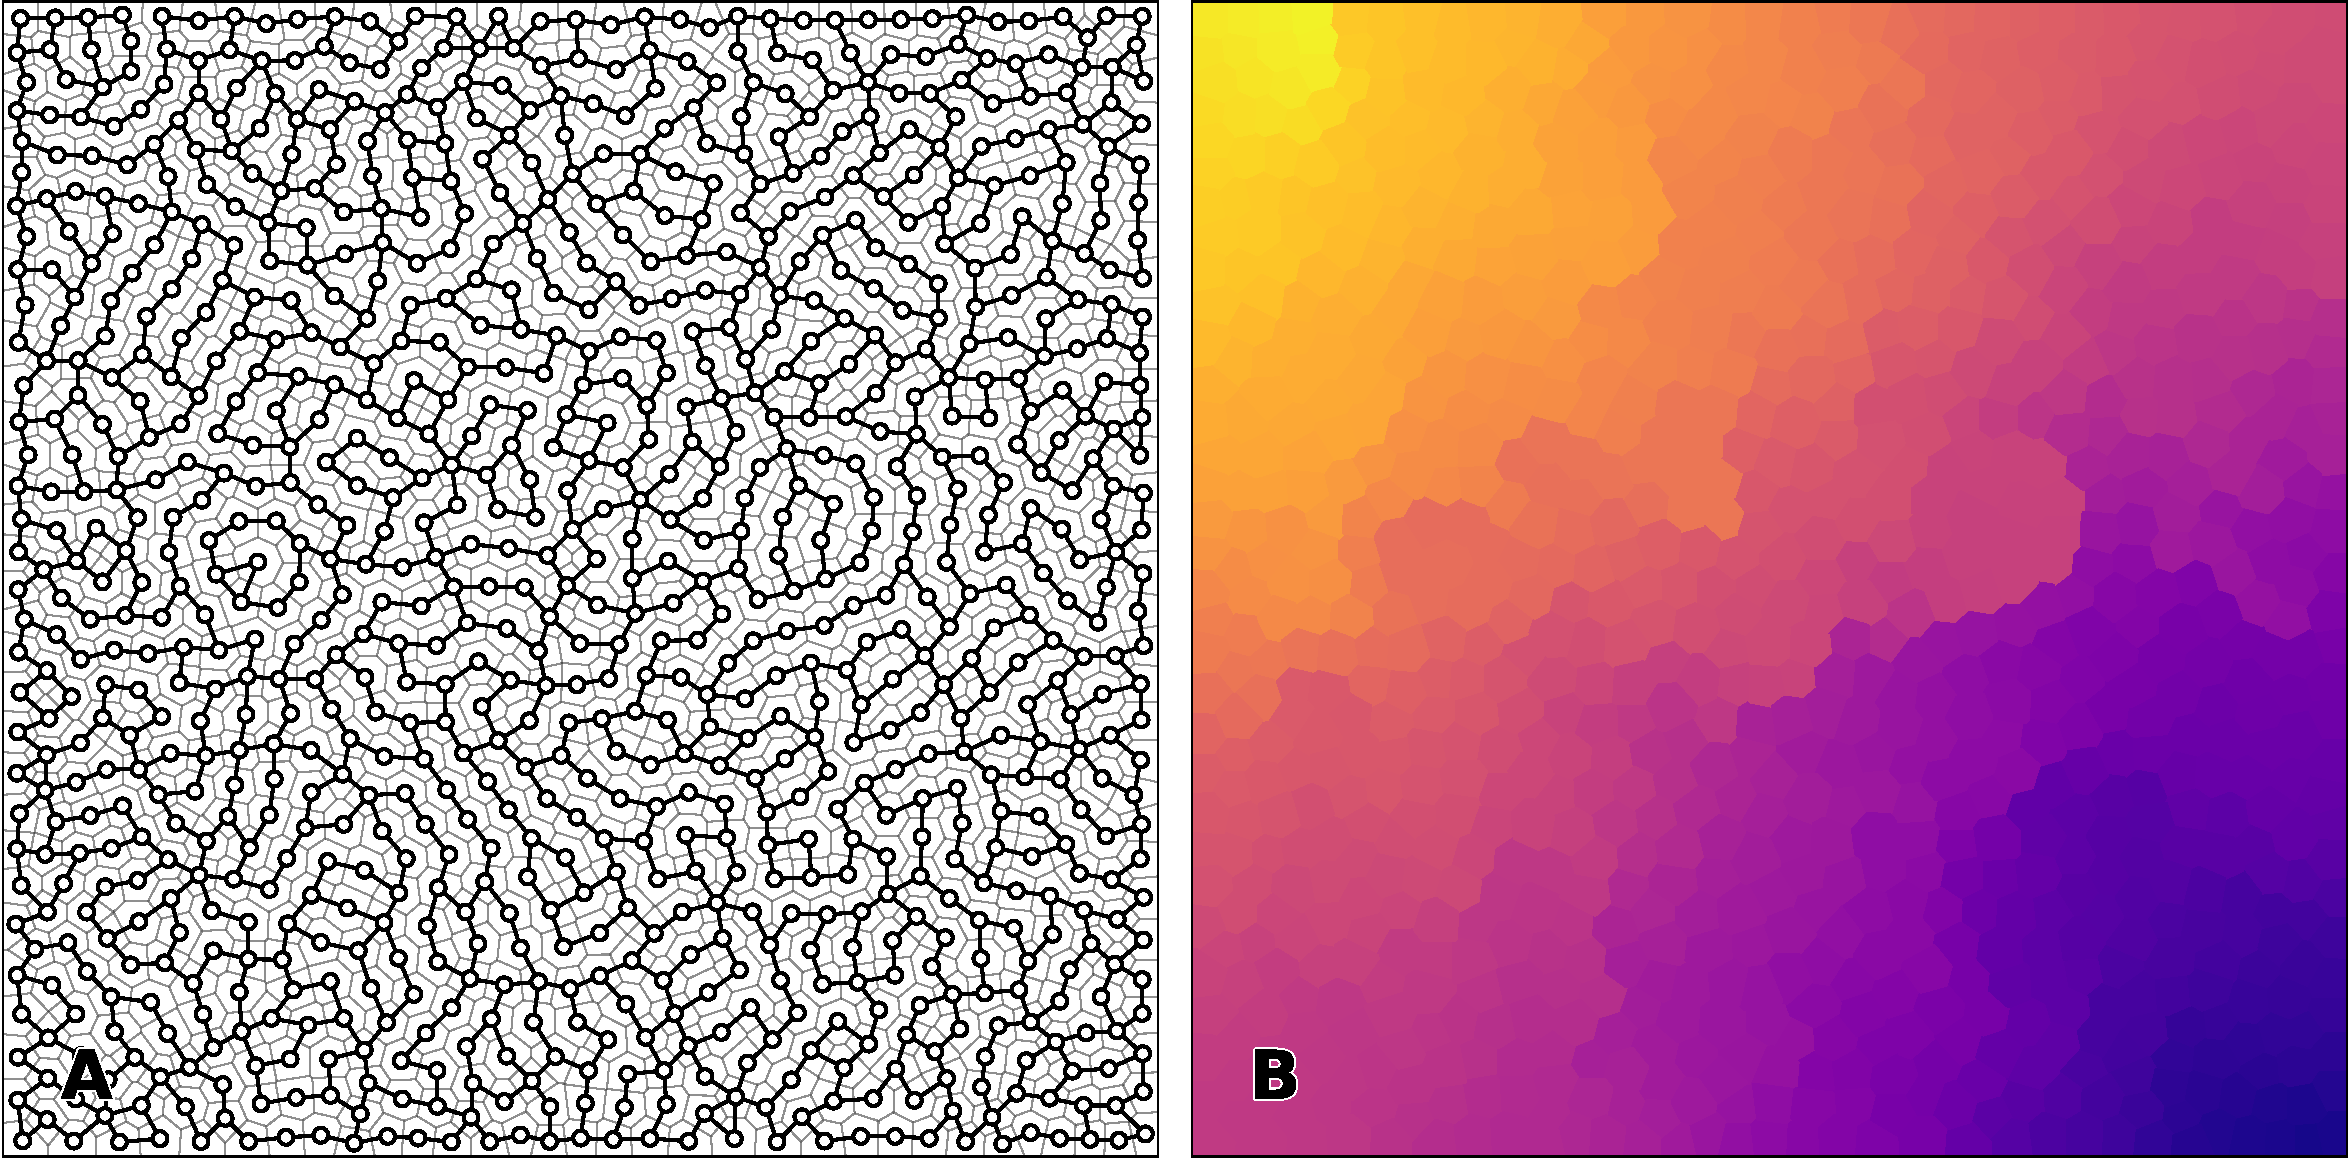
\includegraphics[width=\columnwidth]{figures/vsom-scalar-1.pdf}

  \vspace{2mm}
  
  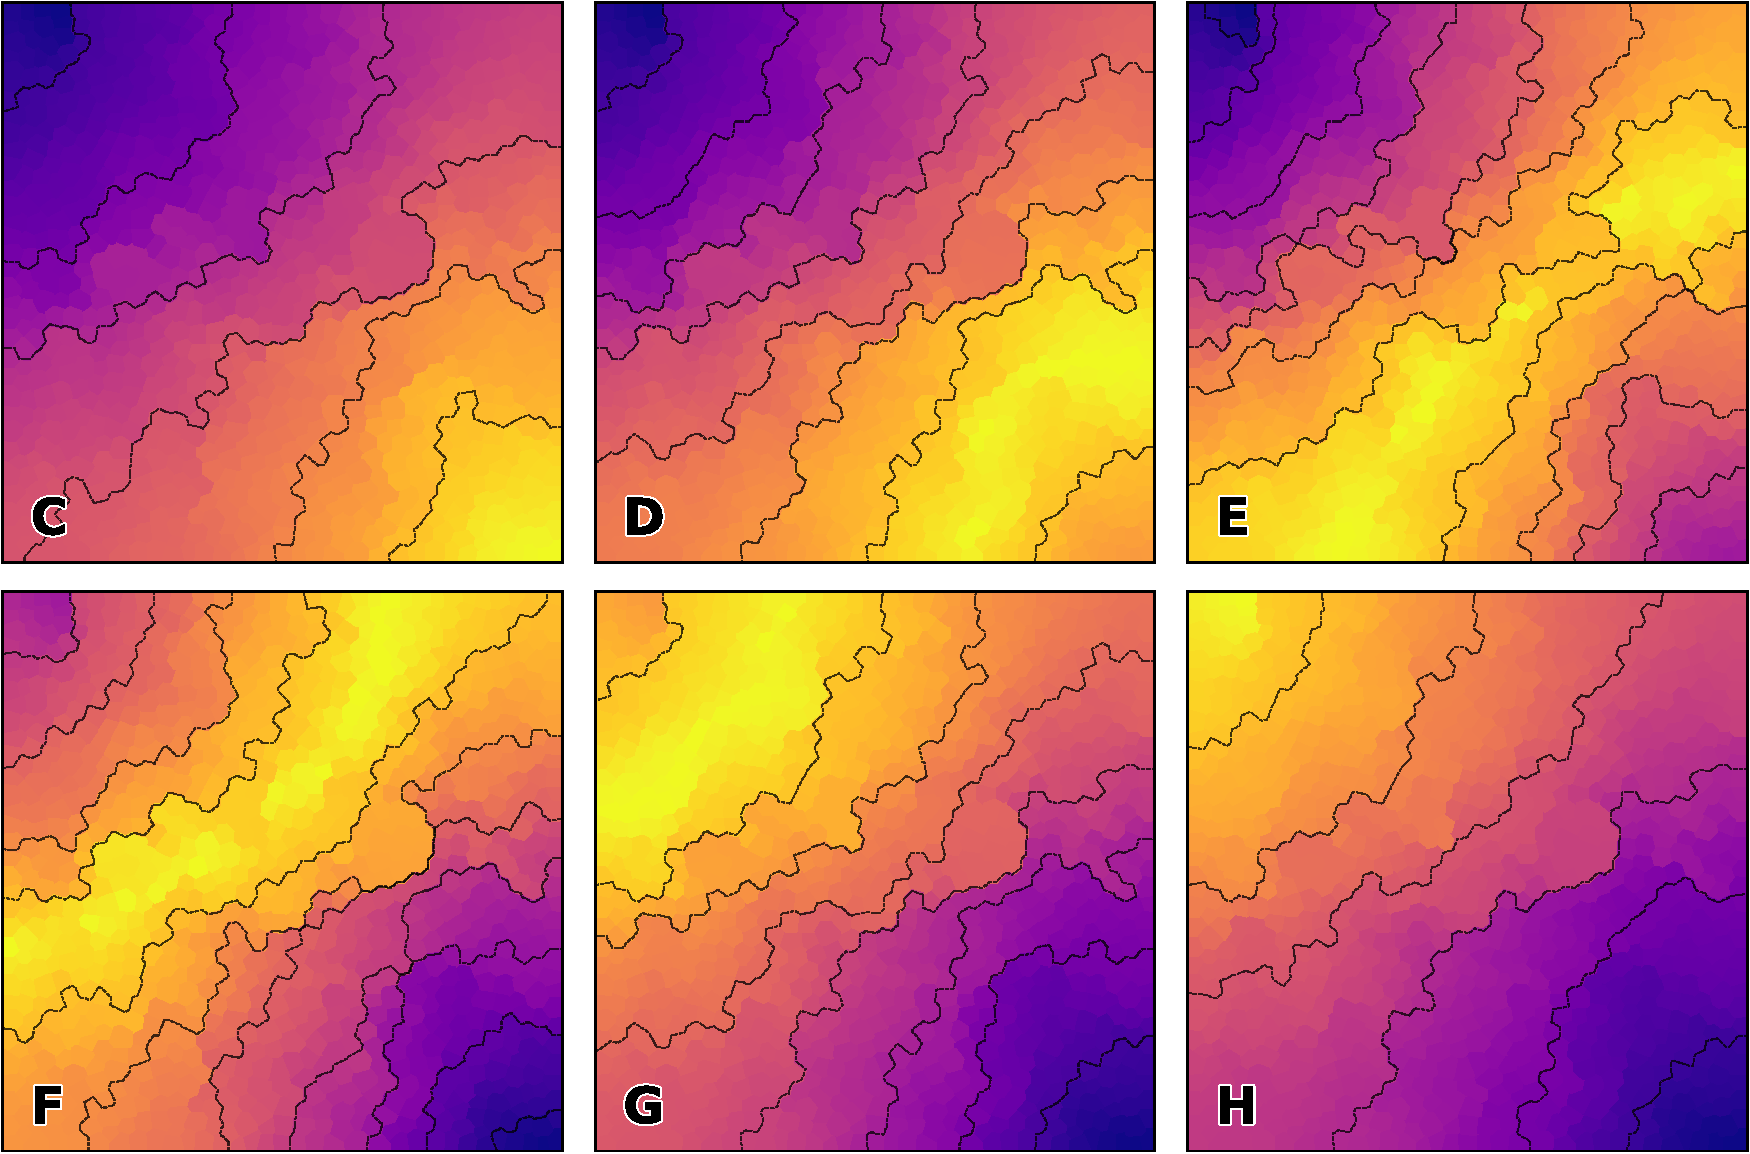
\includegraphics[width=\columnwidth]{figures/vsom-scalar-2.pdf}

  \vspace{2mm}
  
  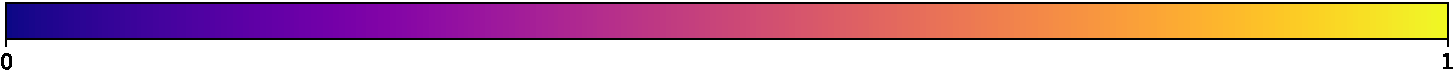
\includegraphics[width=\columnwidth]{figures/colormap.pdf}
  
  \caption{Voronoidal SOM made of $1024$ neurons with a $2$-nearest neighbors
    induced topology. Model has been trained for $25,000$ epochs on random
    uniform scalars drawn from $[0, 1]$. \textbf{A} Map topology in neural
    space. \textbf{B} Map prototypes displayed in neural space using Voronoi
    cells (whose color indicates prototype according to colormap). \textbf{C to
      H} Map activity for six consecutive scalars on the line $[0, 1]$
    (\textbf{C}:0.0, \textbf{D}:0.2, \textbf{E}: 0.4, \textbf{F}:0.6,
    \textbf{G}:0.8, \textbf{H}:1.0).}
    \label{fig:one-dim}
\end{figure}

\begin{figure}
  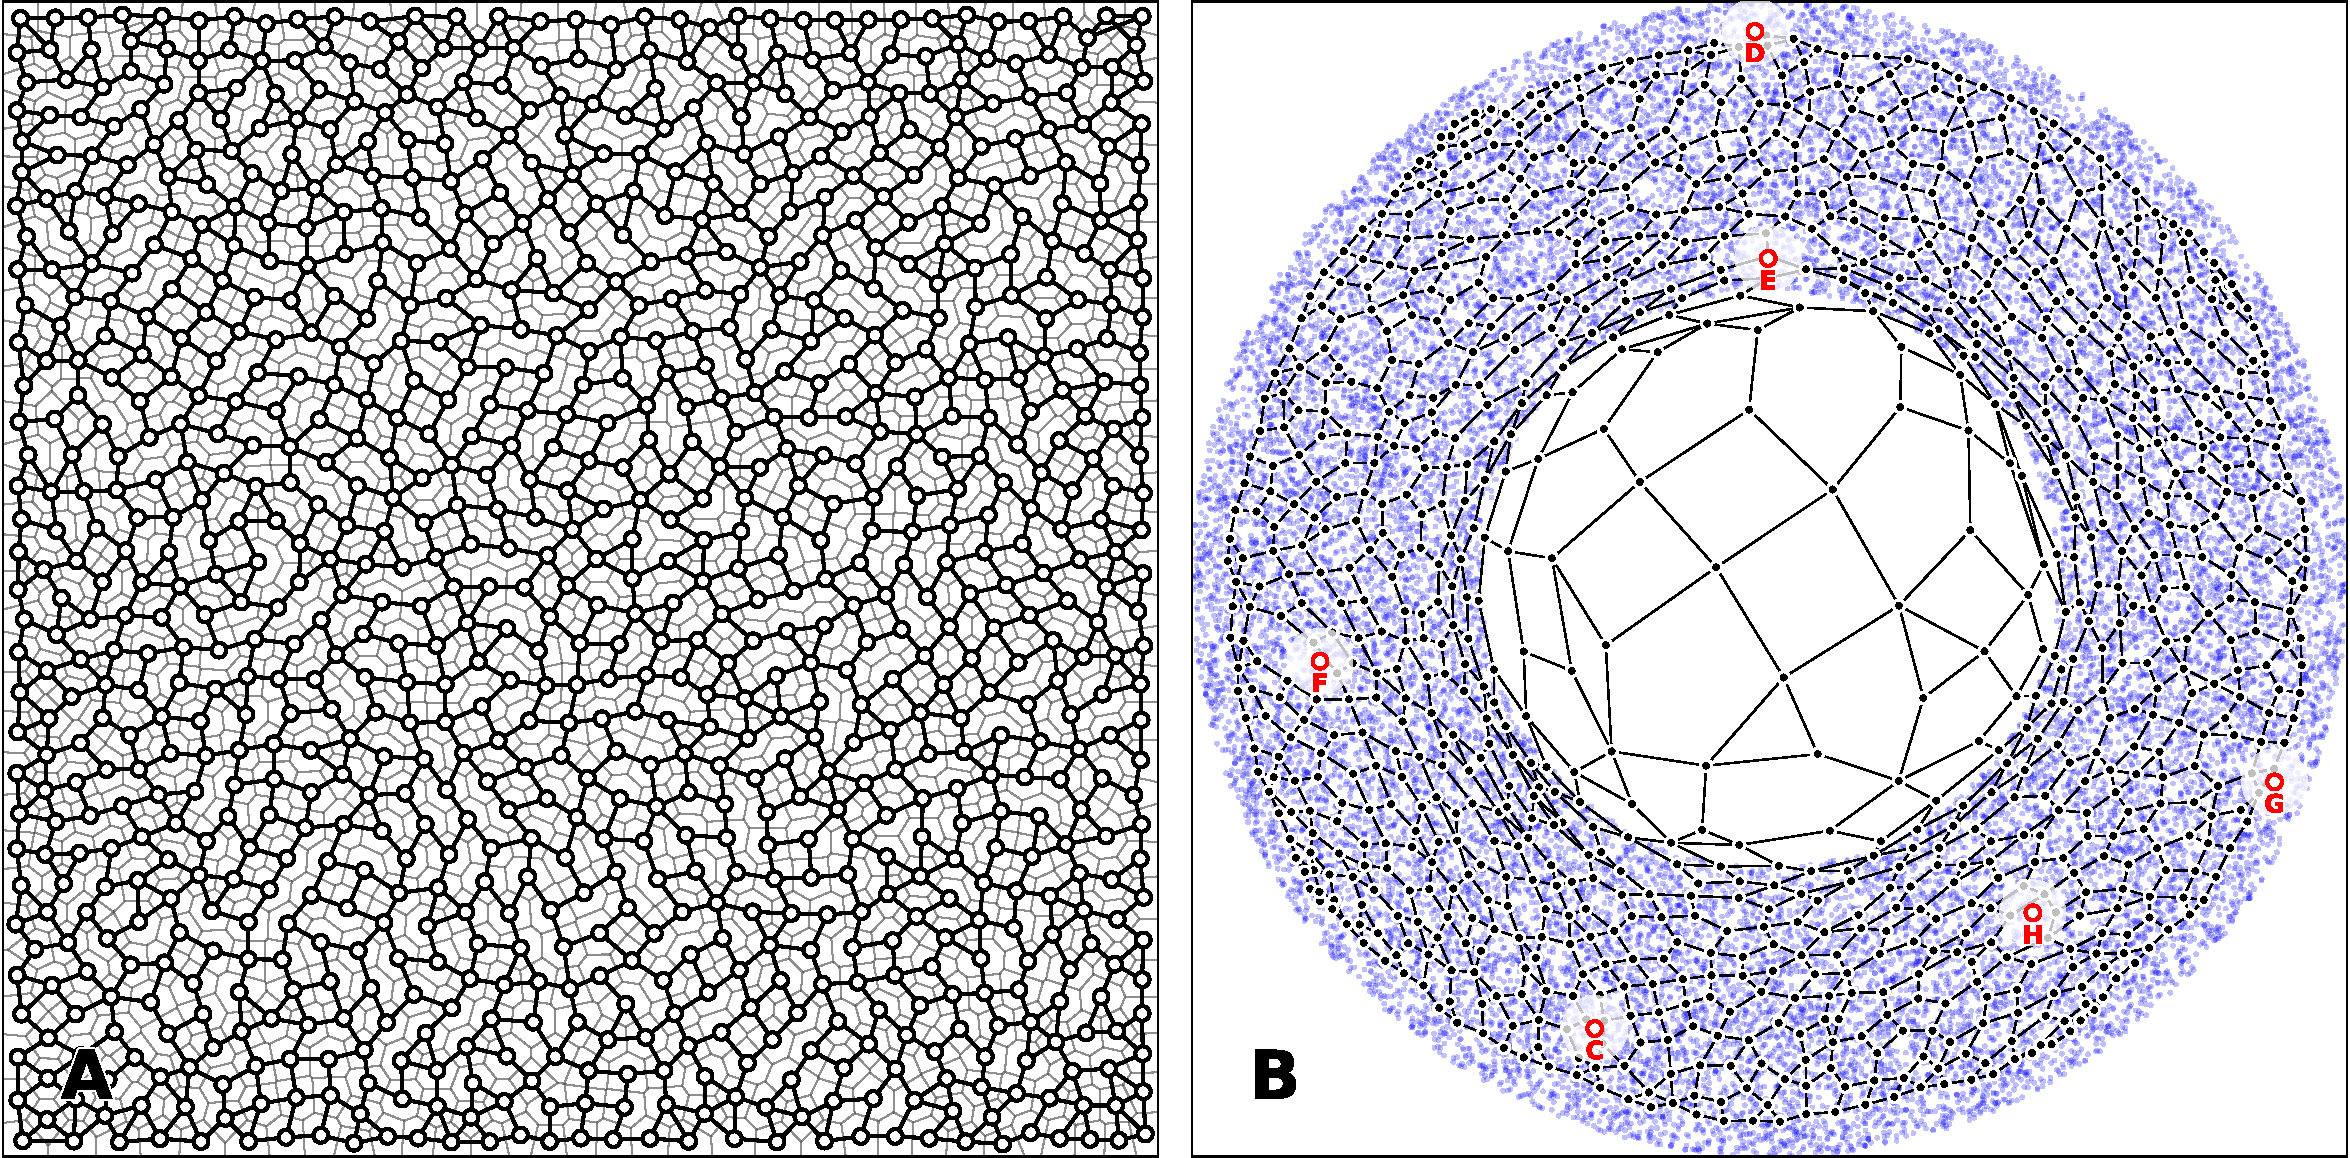
\includegraphics[width=\columnwidth]{figures/vsom-spatial-1.pdf}

  \vspace{2mm}
  
  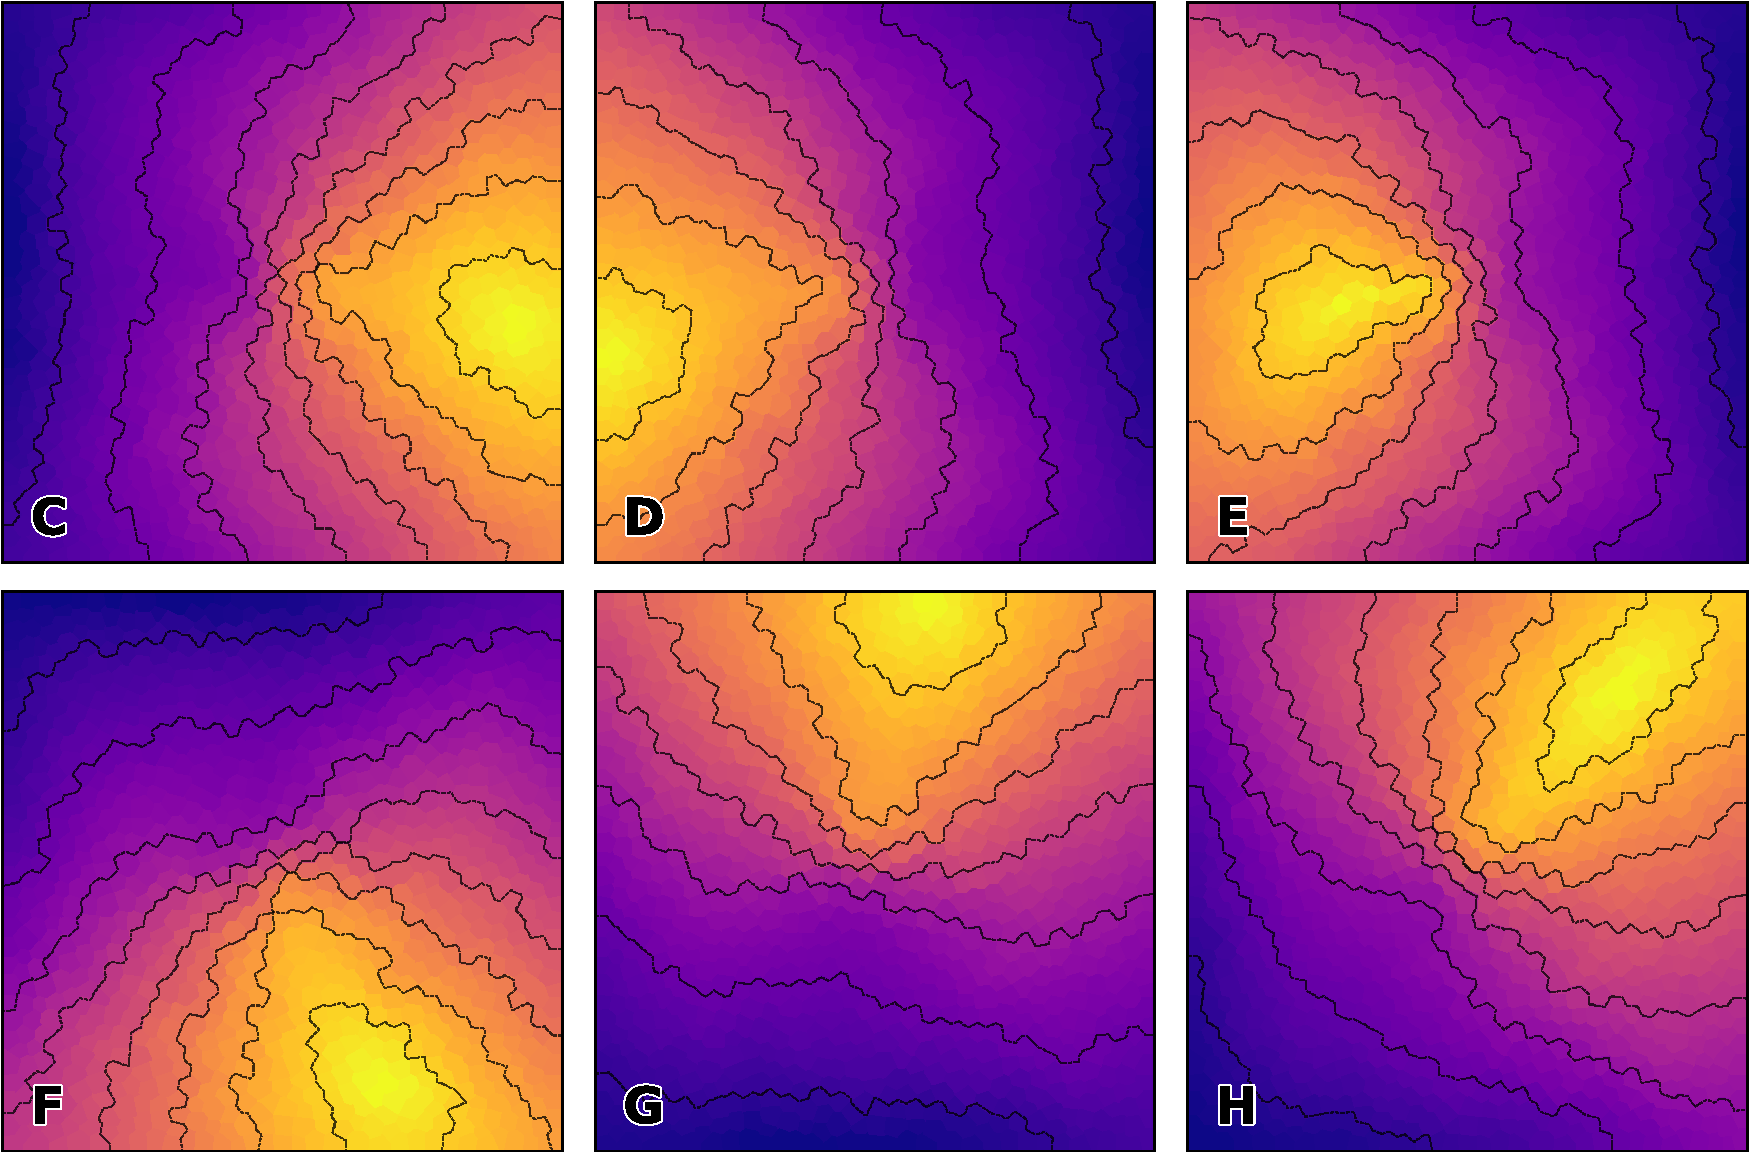
\includegraphics[width=\columnwidth]{figures/vsom-spatial-2.pdf}

  \vspace{2mm}

  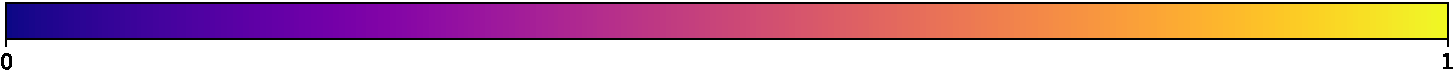
\includegraphics[width=\columnwidth]{figures/colormap.pdf}
  \caption{Voronoidal SOM made of 1003 neurons with a 3-nearest neighbors
    induced topology. Model has been trained for 25,000 epochs on random
    samples inside a torus. \textbf{A} Map topology in the neural
    space. \textbf{B} Map prototypes displayed in data space, blue points are
    the actual samples. \textbf{C to H} Map activity for some random data
    (shown on subplot \textbf{B}).}
    \label{fig:annulus}
\end{figure}


\subsection{High-dimensional data}

\subsubsection{Two-dimensional data}

A two-dimensional map usually maps relatively easy one-dimensional data as 
we have already shown in the previous paragraph. Next, we investigate the
performance and behavior of a two-dimensional map on learning two-dimensional
representations. First, we train the SOM algorithm on $25000$ two-dimensional 
points drawn from a uniform distribution of an annulus in $[0, 1]\times[0, 1$],
and second, on a two-dimensional artwork by Mucha (The Spring). In the latter
case, the image is converted to grayscale and its pixel values are normalized
to $[0, 1]$. For the artwork we train the SOM on $50000$ data points. 

As we have already described, first we place the neurons on the appropriate
positions on neural space with respect to the topology provided by a blue noise
distribution. The map topology for the annulus is shown in
Figure~\ref{fig:annulus}{\bfseries \sffamily A} and for the two-dimensional
picture in Figure~\ref{fig:mucha}{\bfseries \sffamily A}. Hence, we proceed to
the learning part by training the SOM algorithm over the two data sets for 
$25000$ epochs.

Figure~\ref{fig:annulus}{\bfseries \sffamily B} shows the mapping produced by
the SOM algorithm~\ref{algo:vsom} trained on the annulus data set. As we
observe the map covers the input space with higher density within the annulus,
where the input data points live, and a lower density within the hole of
annulus. Panels~\ref{fig:annulus}{\bfseries \sffamily C}-{\bfseries \sffamily H}
display the responses of six neurons (see the red annotated points in
panel~\ref{fig:annuslus}{\bfseries \sffamily B}) to a stimulus derived from 
the discretization of $[0, 1]\times [0, 1]$. The responses of these neurons
are well organized and reflect their receptive fields.

Next, we trained the SOM on Mucha's data set (see 
figure~\ref{fig:mucha}{\bfseries \sffamily A}) for $25000$ epochs. Again, we
calculated the positions of neurons via a blue noise distribution \gid{TODO Figure
needs to be fixed, it's not correct. Add more text here explaining better
what's going on.}

\begin{figure}
  \setlength{\fboxsep}{0pt}%
  \setlength{\fboxrule}{.25pt}%

  \fbox{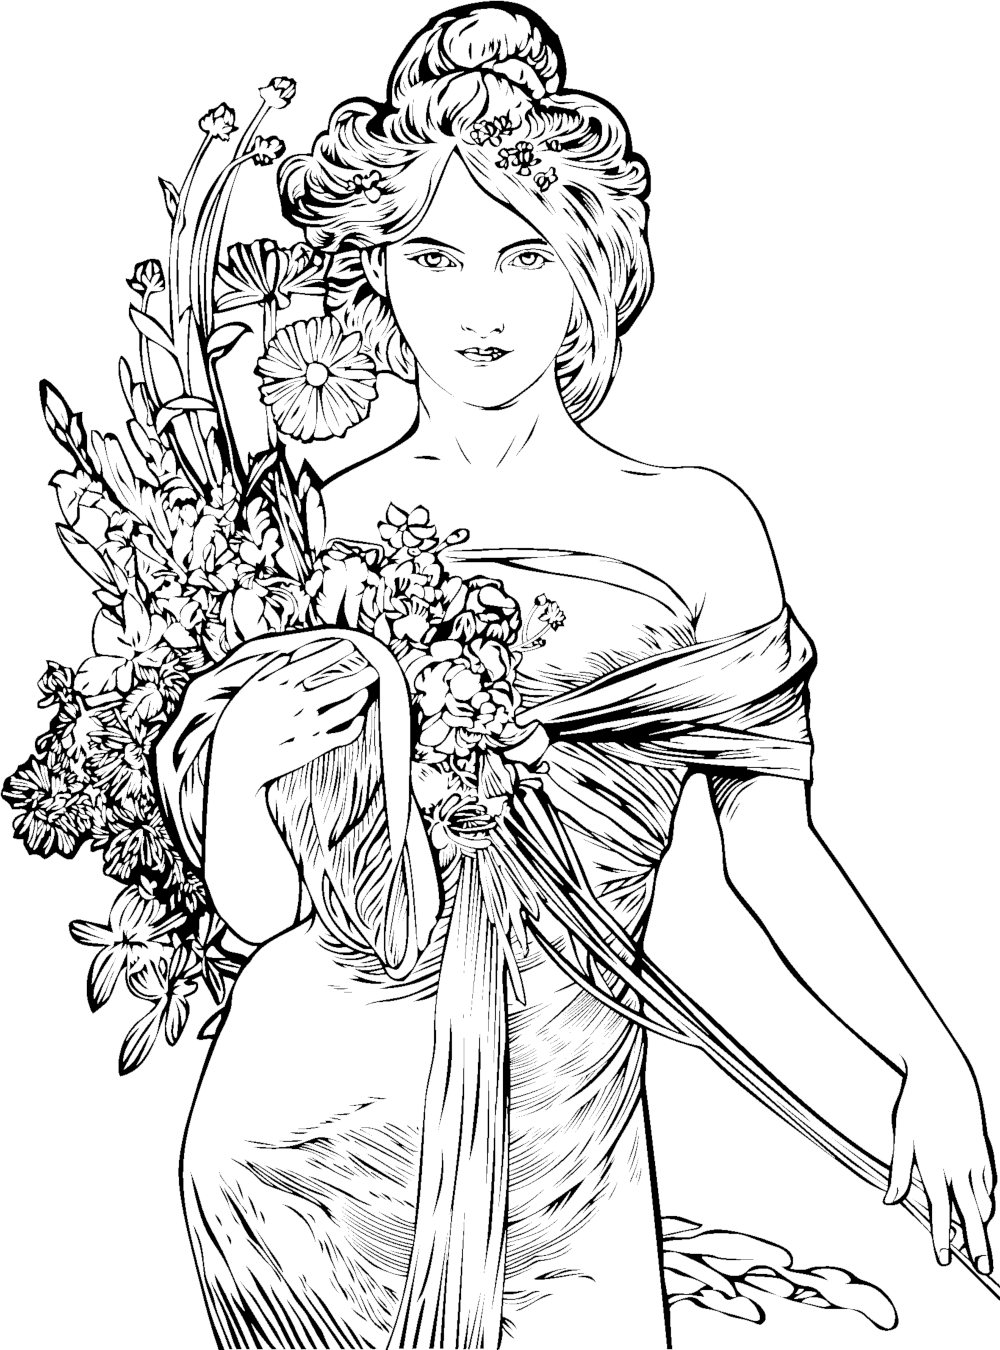
\includegraphics[height=5.1cm]{figures/mucha.png}}
        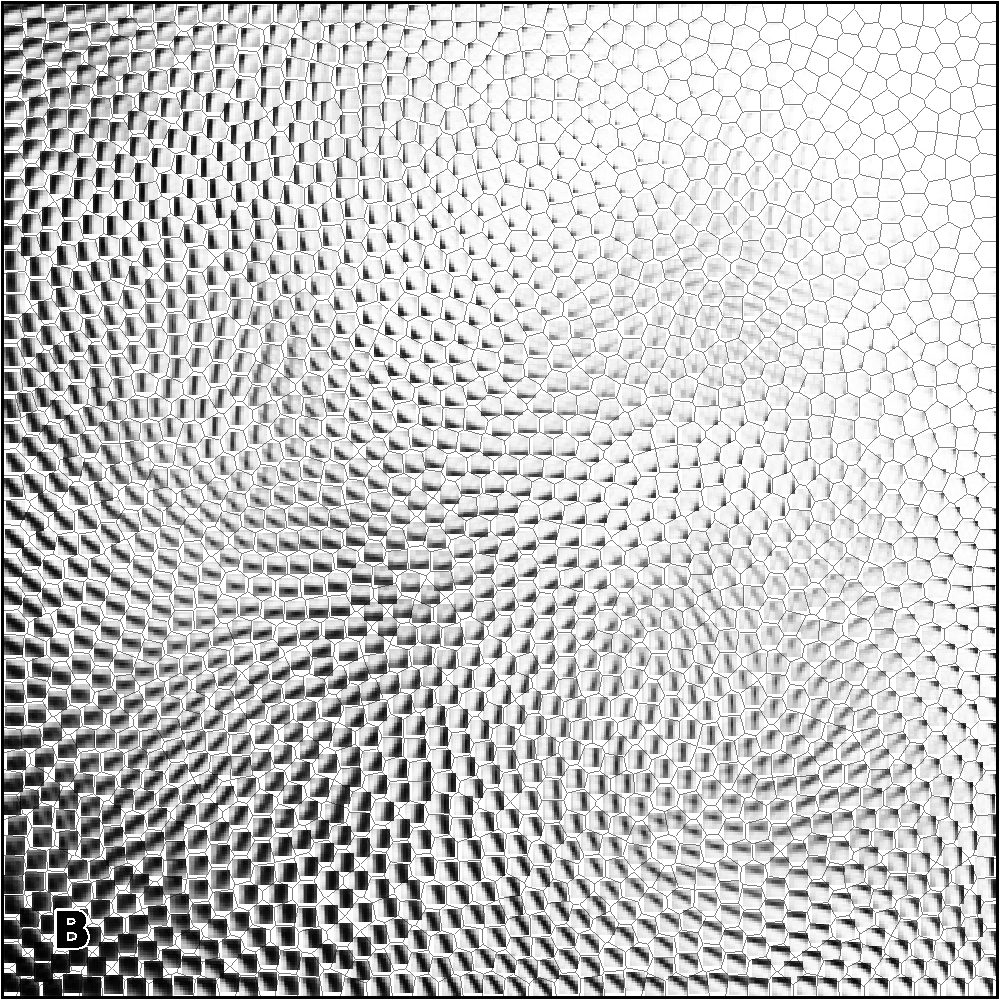
\includegraphics[height=5.1cm]{figures/vsom-image.pdf}
  \fbox{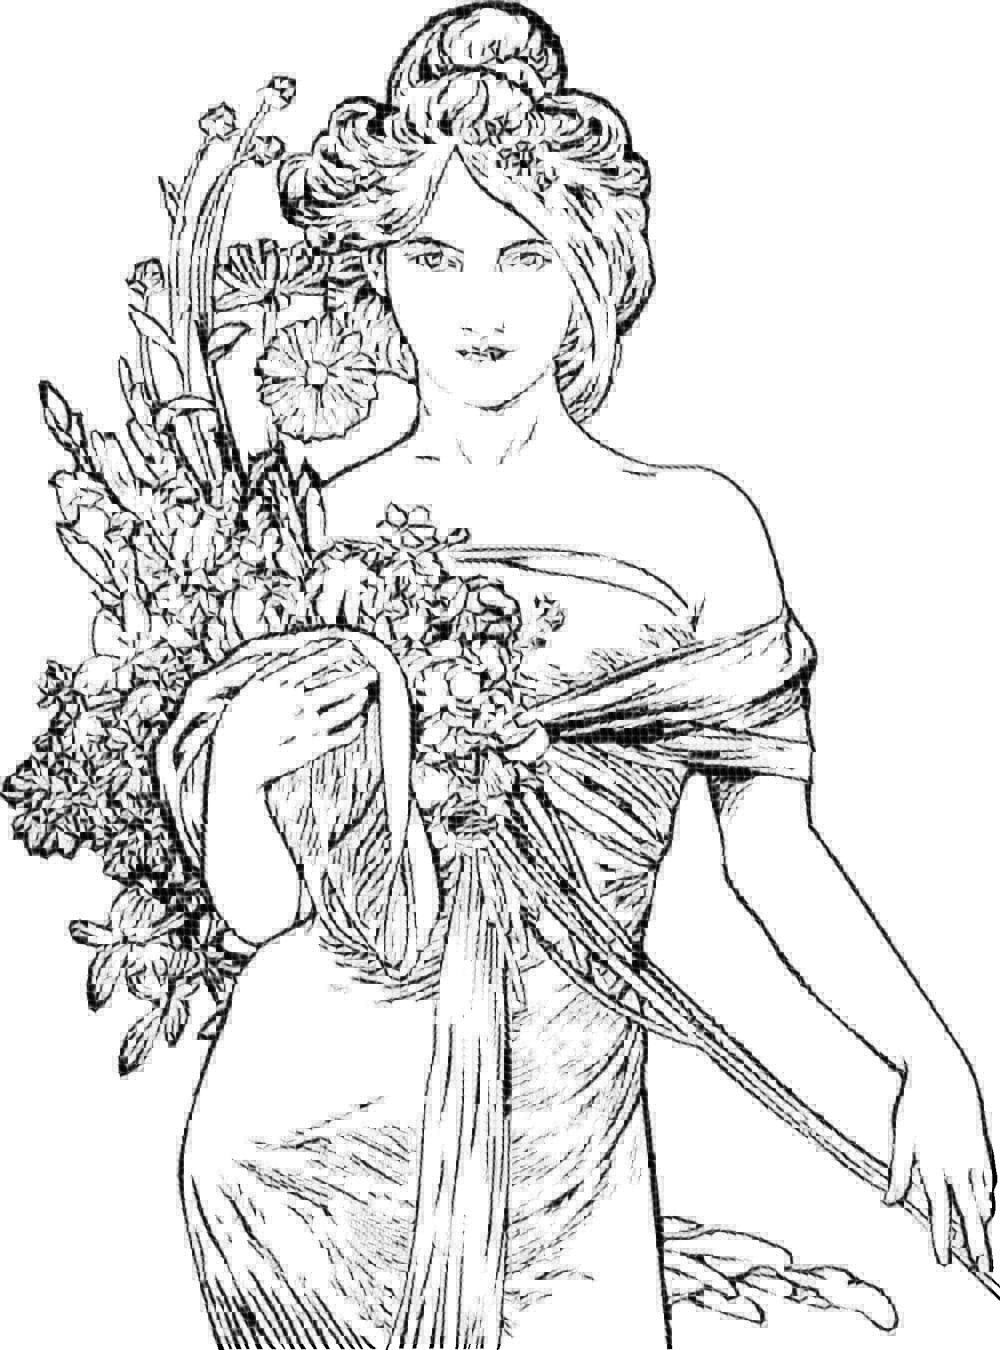
\includegraphics[height=5.1cm]{figures/mucha-vsom.png}}

%  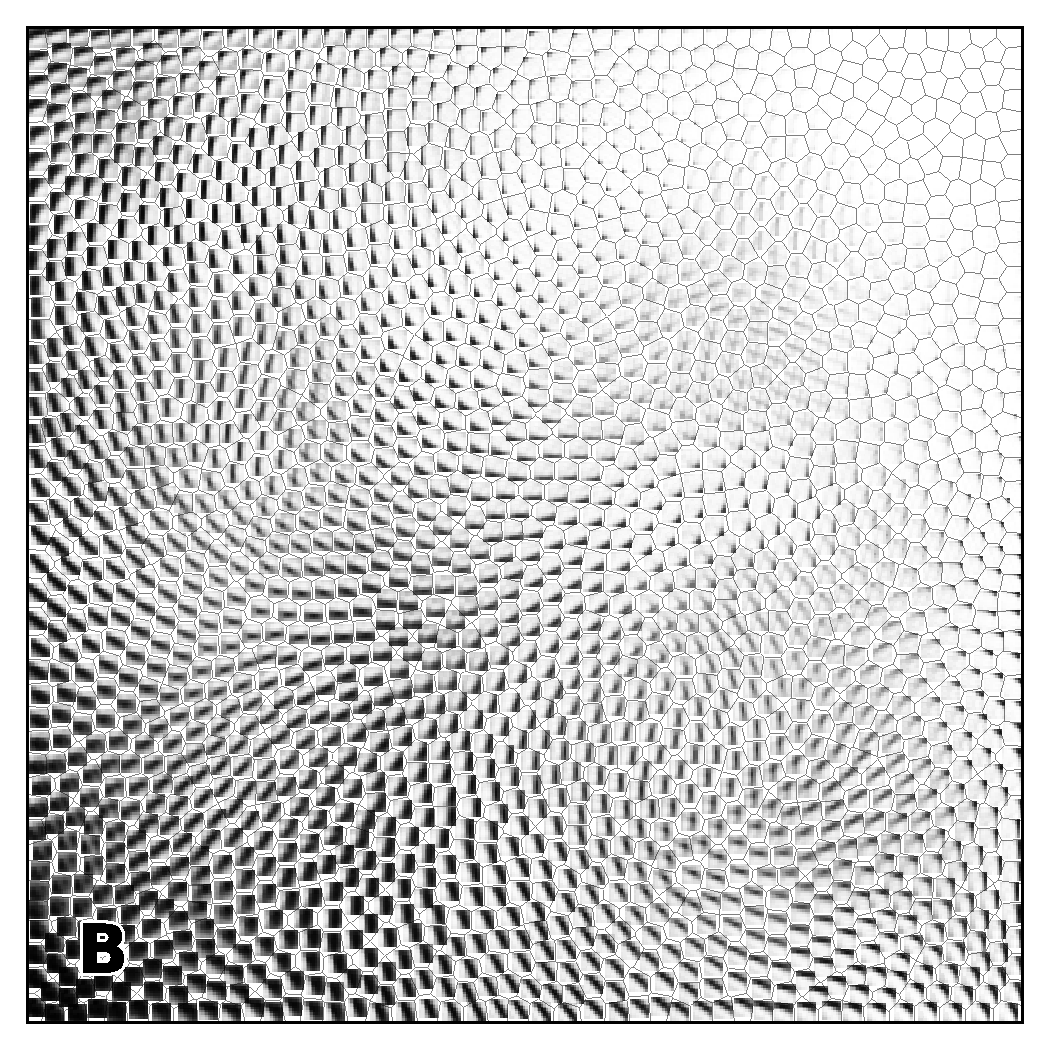
\includegraphics[width=\textwidth]{figures/vsom-image-1.pdf}
  
  \vspace{2mm}

  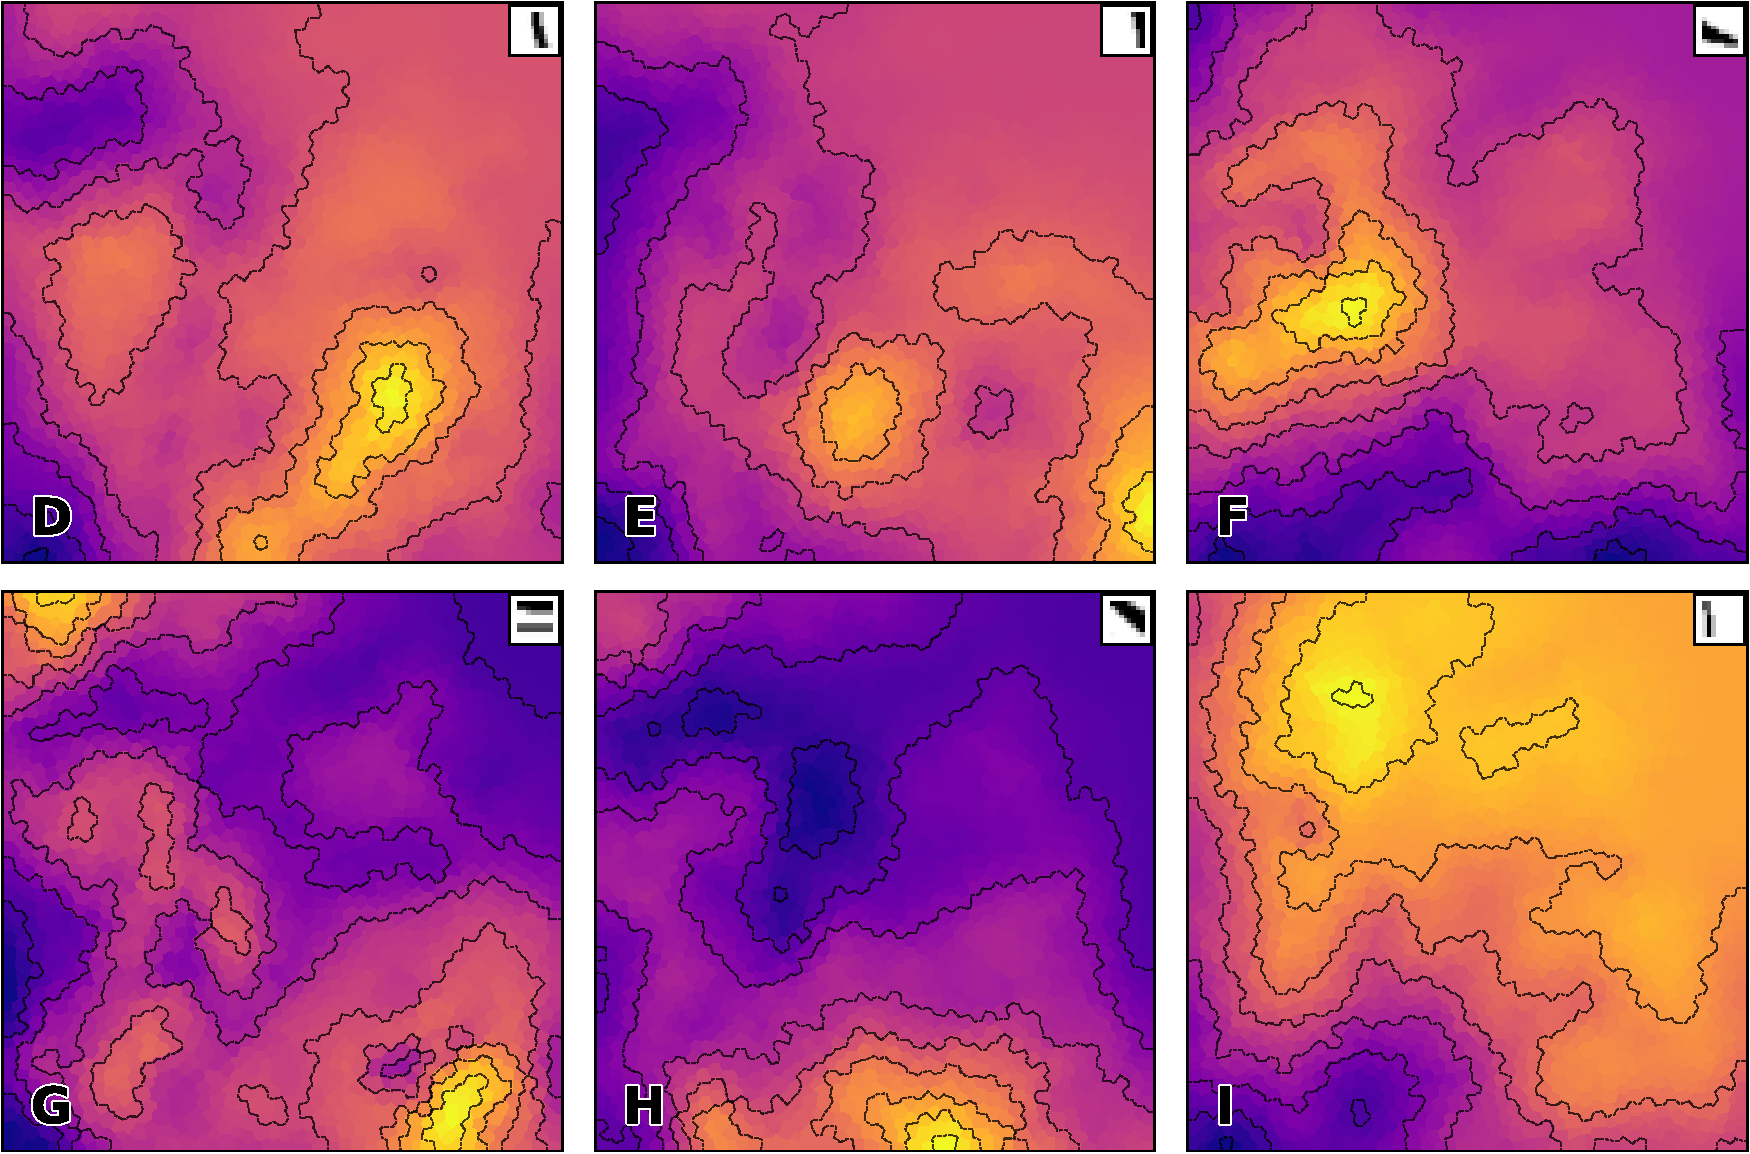
\includegraphics[width=\textwidth]{figures/vsom-image-2.pdf}

  \caption{Voronoidal SOM made of 1003 neurons with a 2-nearest neighbors
    induced topology. Model has been trained for 10,000 epochs on random
    uniform scalars in [0,1]. \textbf{A} Map topology in the neural
    space. \textbf{B} Map prototypes displayed in neural space using Voronoi
    cells (whose color indicates prototype according to colormap). \textbf{C to
      H} Map activity for some random data (\textbf{C}:0.0, \textbf{D}:0.2,
    \textbf{E}: 0.4, \textbf{F}:0.6, \textbf{G}:0.8, \textbf{H}:1.0).}
    \label{fig:mucha}
\end{figure}


\subsubsection{Three-dimensional data}

For the three-dimensional experiment we $50000$ draw three-dimensional points
from a uniform distribution $\mathcal{U}([0, 1]\times [0, 1]\times [0, 1])$
(the cloud points form a cube in $\mathbb{R}^3$). The map is a two-dimensional
manifold and thus the required task it to map the three-dimensional vectors 
to the two-dimensional neural space. Once again we place the neurons on the
two-dimensional neural space based on the sampling of a blue noise distribution
and the induced topology is illustrated in Figure~\ref{fig:three-dim}{\bfseries \sffamily A}.
The learning algorithm~\ref{algo:vsom} runs for 
$25000$ epochs over the three-dimensional vectors and after convergence we 
obtain the map with the prototypes shown in Figure~\ref{fig:three-dim}{\bfseries \sffamily B}.
Each color represents a different face of the three-dimensional cube (a cube
has six faces so we obtain mainly six colors) and we observe that the SOM
has mapped the three-dimensional cube on a two-dimensional neural space. The 
continuity and grouping of the colors indicates that the receptive fields of 
the neurons have been established properly. We illustrate this phenomenon in 
panels~\ref{fig:three-dim}{\bfseries \sffamily C}-{\bfseries \sffamily H}, 
where the response of six different neurons (see the annotation in
panel~\ref{fig:three-dim}{\bfseries \sffamily B}). The dark blue color
indicates values close to zero and the yellow color represents values close to
one.

\begin{figure}
  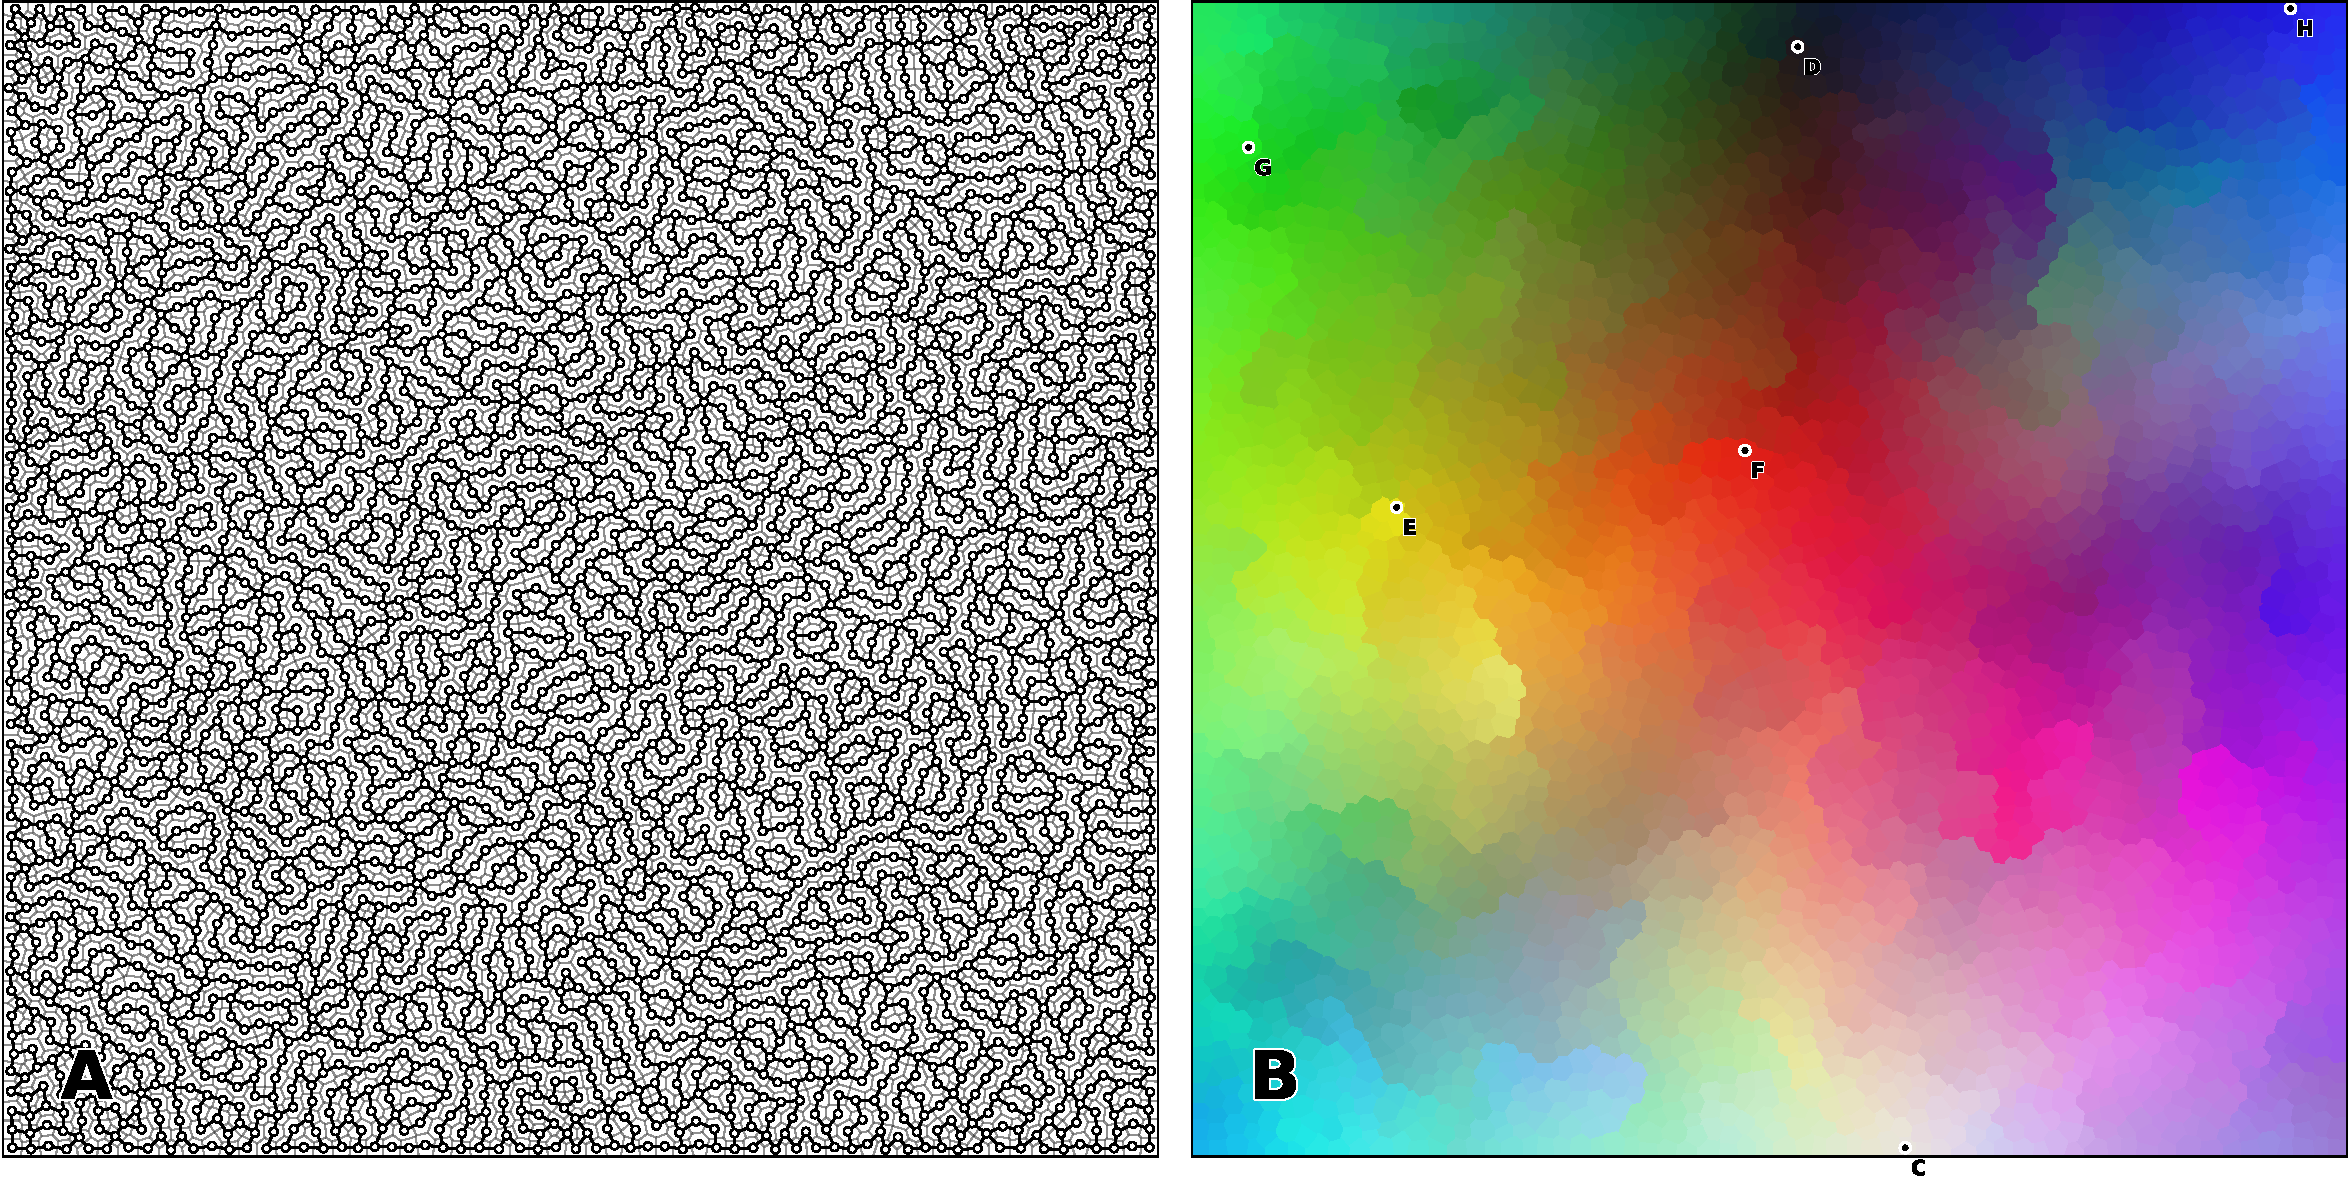
\includegraphics[width=\columnwidth]{figures/vsom-colors-1.pdf}

  \vspace{2mm}
  
  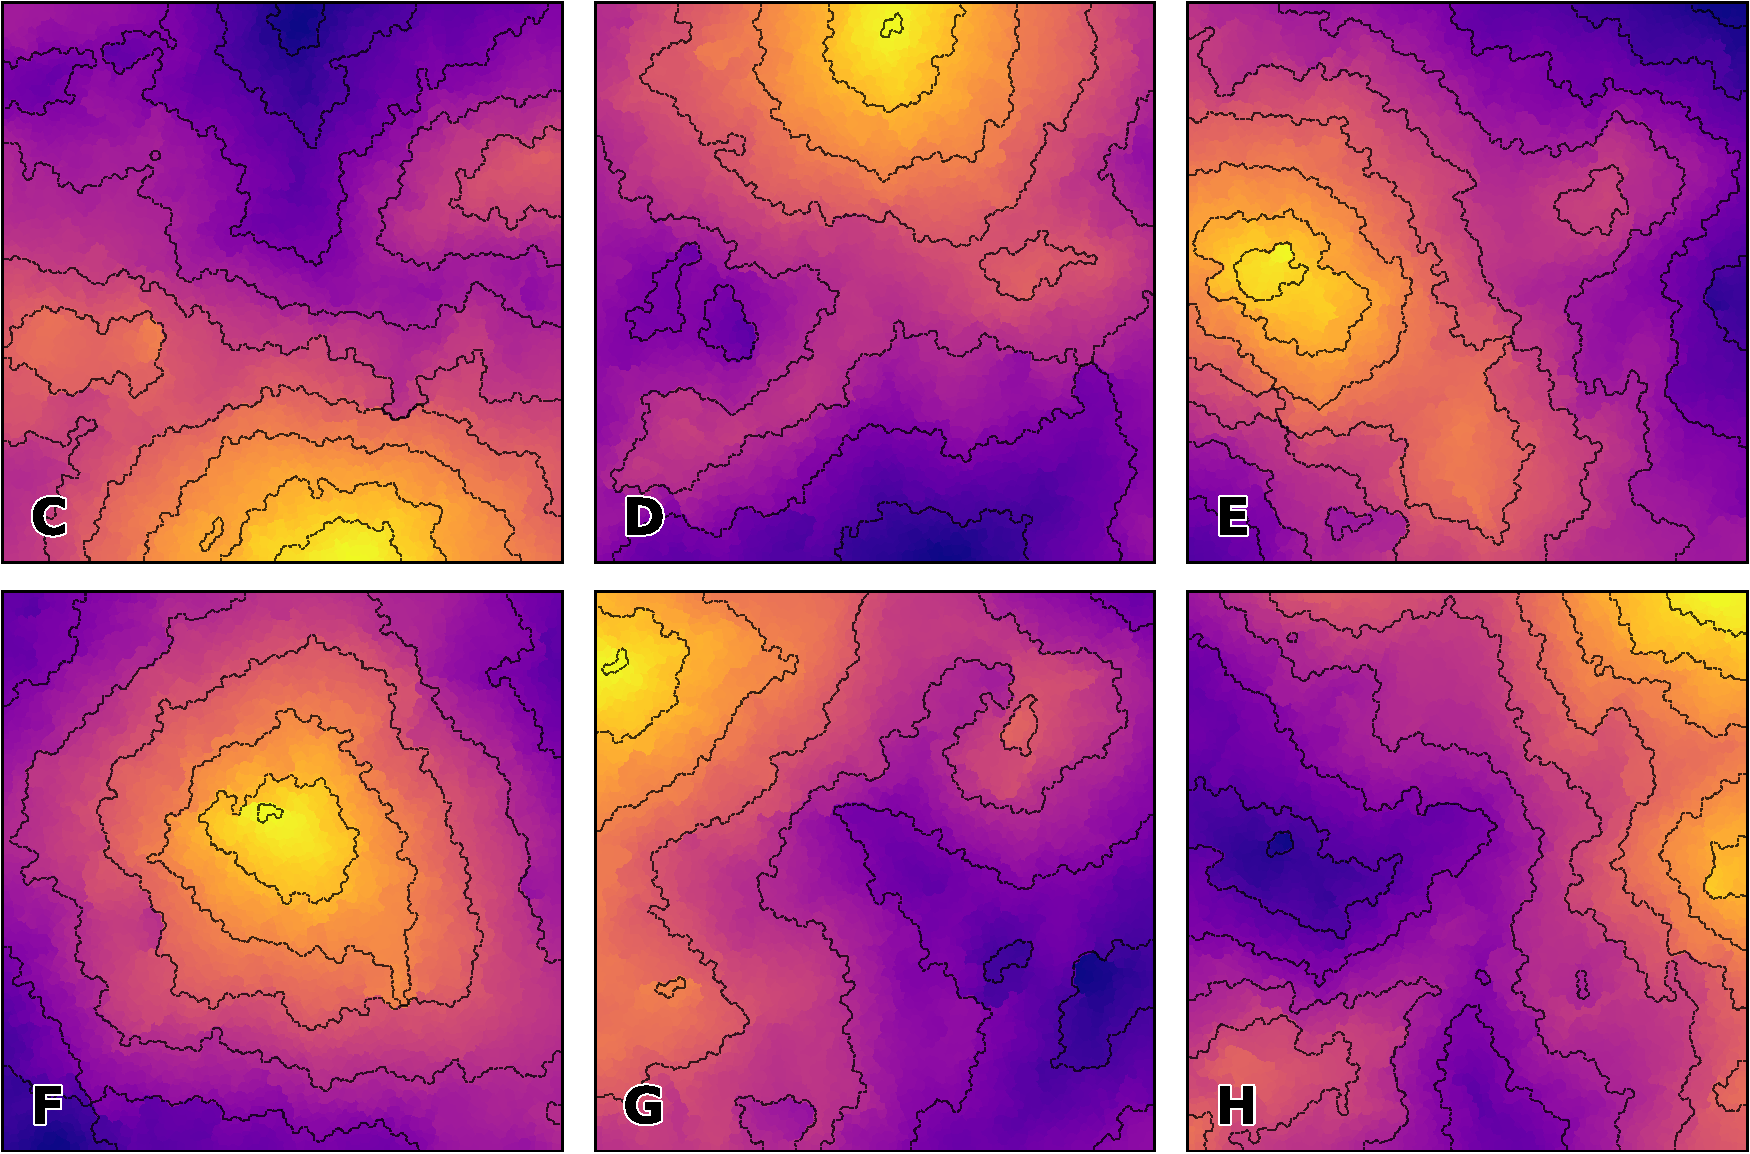
\includegraphics[width=\columnwidth]{figures/vsom-colors-2.pdf}

  \vspace{2mm}

  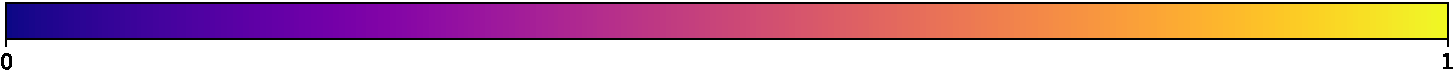
\includegraphics[width=\columnwidth]{figures/colormap.pdf}

  \caption{}
  \label{fig:three-dim}
\end{figure}



\subsection{Reorganization}

The final and most challenging experiment is to test how the proposed SOM
algorithm handles degenerative cases, where either neurons
die out (ablation) or new units are added to the map (addition). 
Figure~\ref{fig:CVT} {\bfseries \sffamily A} illustrates an example of a
well-formed neural space (black outlined discs), an ablation
(red disks) and an addition (black dots). In ablation units colored in red are
removed from the map and in addition neurons indicated by black dots are
added to the map. 
For both ablation and addition we can apply a LLoyd relaxation scheme to 
achieve a new quasi centroidal Voronoi tesselation. Figures~\ref{fig:CVT}{\bfseries \sffamily E},
and {\bfseries \sffamily F} depicts the Voronoi tesselations after $100$ 
iterations starting from the initial tesselation pictured by 
panel~\ref{fig:CVT}{\bfseries \sffamily D}. 

Previous studies have shown that after an ablation or addition of units the
map undergoes a reorganization of its neural representations. The immediate 
consequence of a reorganization is the acquisition of new receptive fields. 
When an ablation takes place, unaffected neurons try to recover representations
that got lost due to neurons death. In addition, on the other hand, the surplus
neurons have to get their share of the representations and thus the entire map
undergoes a reorganization.

The induced topology shares similarity with the original
topology (before ablation or addition).
\gid{TODO Add a few more words here. Maybe make a connection to neuroscience facts
about reorganization.}

\begin{figure}
  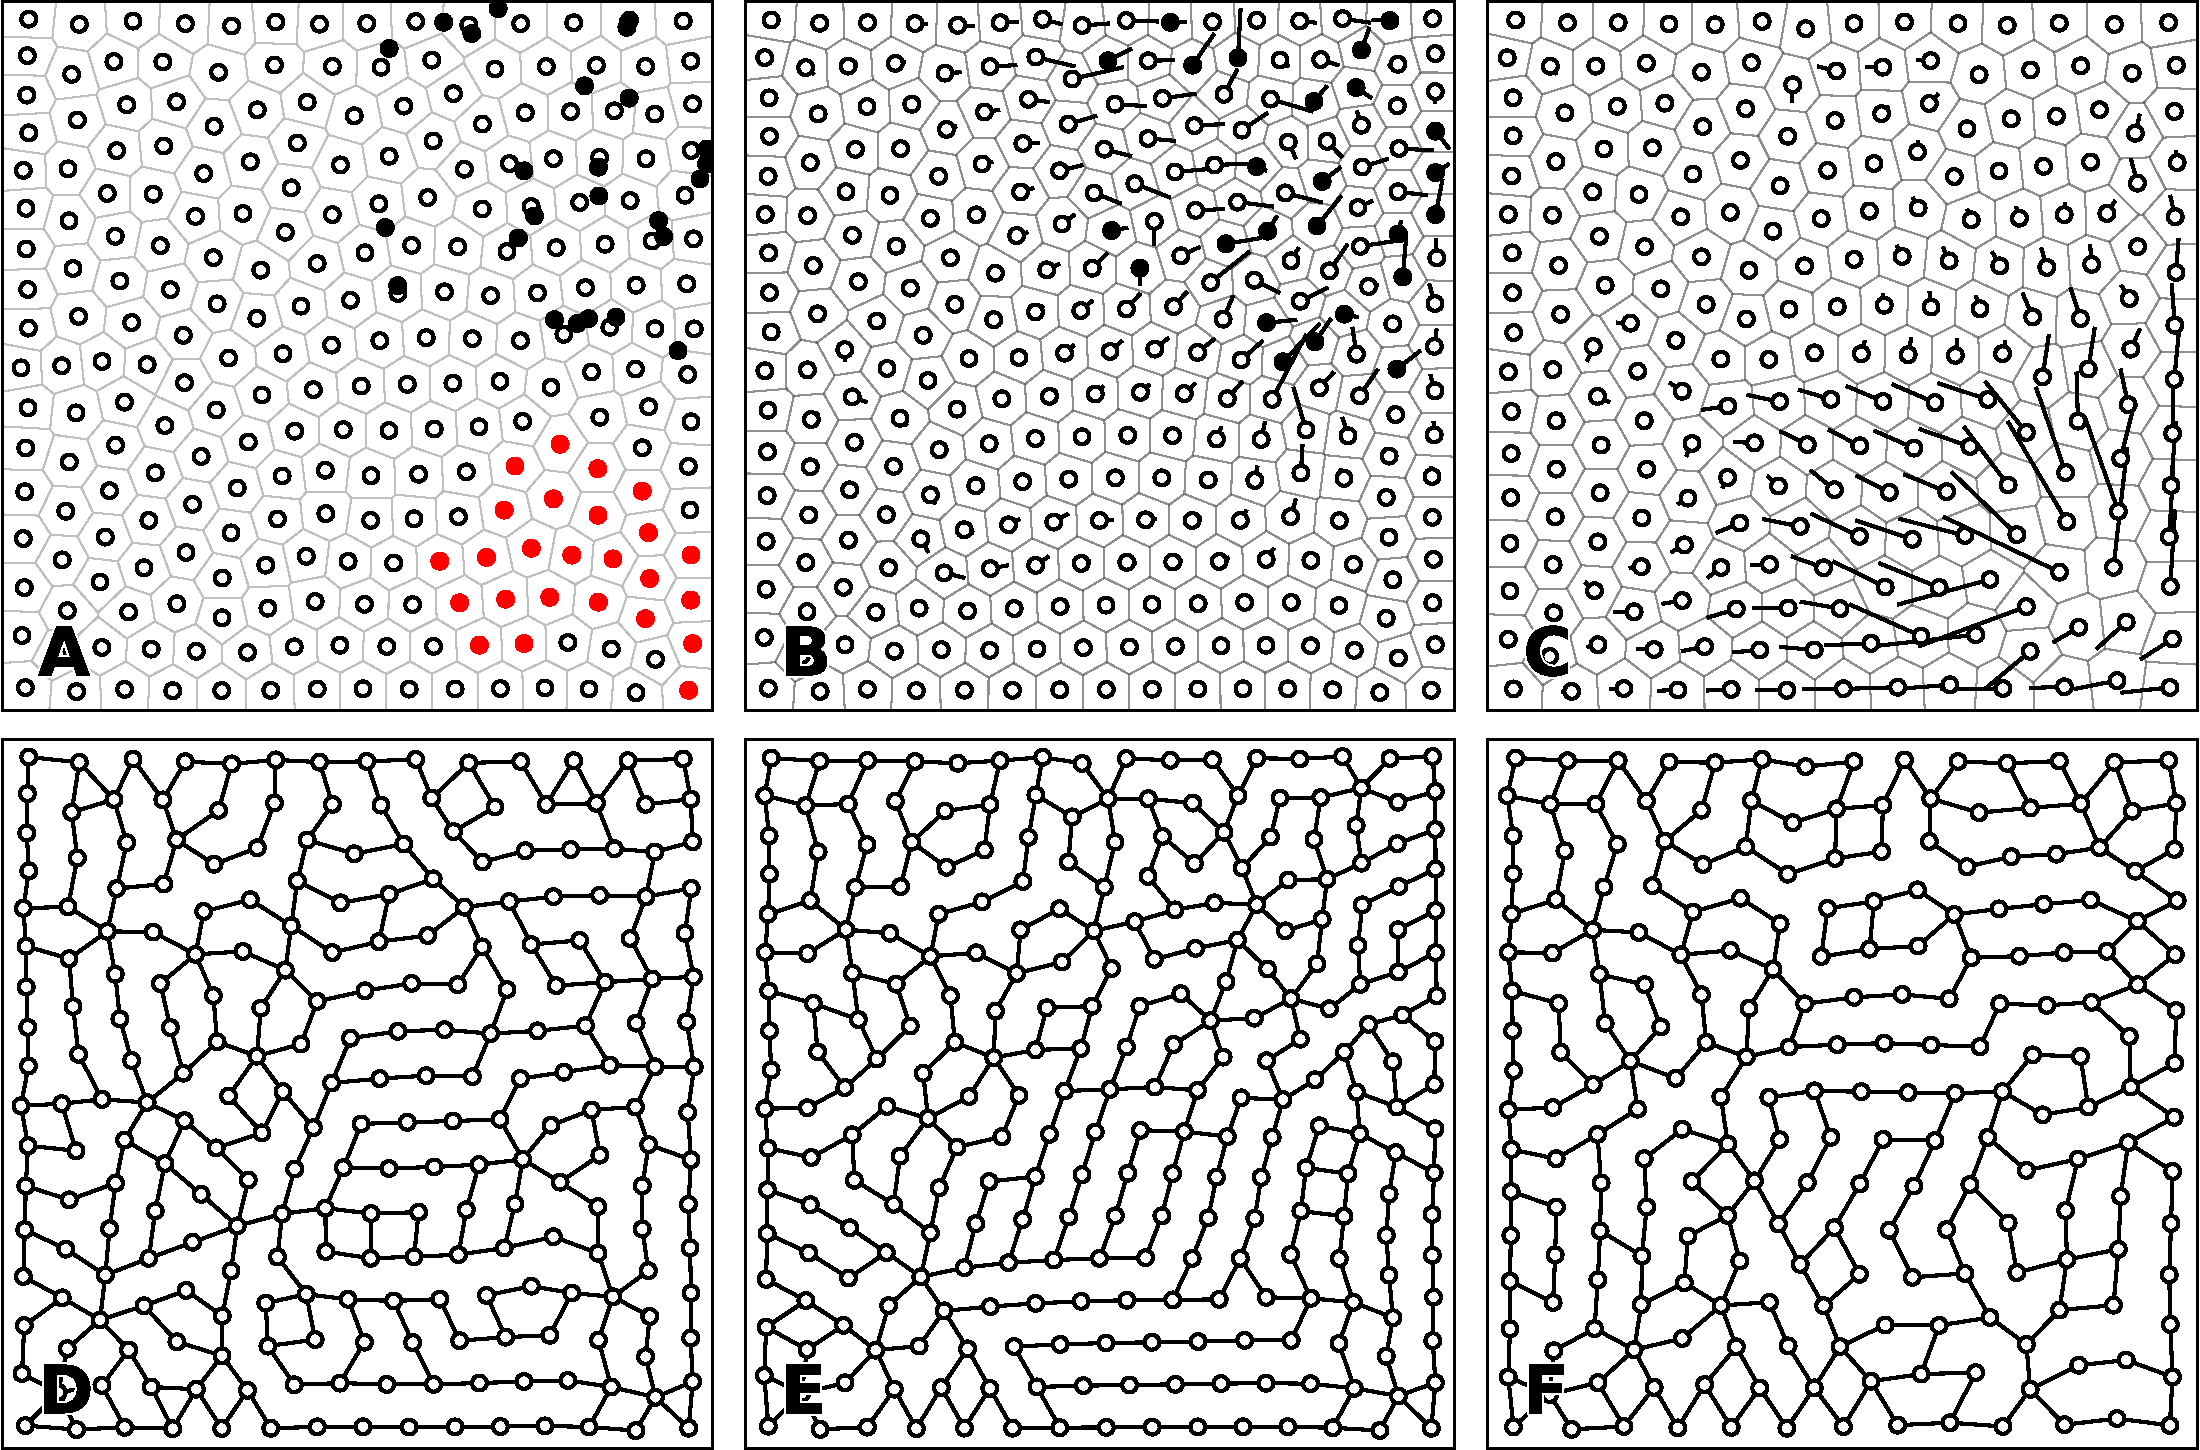
\includegraphics[width=\columnwidth]{figures/vsom-resilience.pdf}
  \caption{\textbf{Reorganization following neural loss or gain.}  An initial
    set of 248 neurons (outlined discs on panel \textbf{A}) has been modified
    with the addition of 25 neurons (black discs) or the removal of 25 neurons
    (red discs). Panels \textbf{B} and \textbf{C} show the final position of
    neurons after 100 iterations of the centroidal Voronoi tesselation. Lines
    shows individual movement of neurons. Panels \textbf{D}, \textbf{E} and
    \textbf{F} show the 2-neighbors induced topology for \textbf{A},
    \textbf{B} and \textbf{C} respectively.}
  \label{fig:CVT}
\end{figure}

\subsubsection*{Ablation}

\subsubsection*{Addition}
